\documentclass[12pt]{report}
\usepackage[utf8]{inputenc}
\usepackage{graphicx}

\title{F21DL: Coursework One}
\author{
	Omkar Gosavi
	\and
	Prashant Sawant
	\and
	Timothy Makobu
}

\date{\today}

\usepackage[backend=biber,style=authoryear-ibid,sorting=ynt]{biblatex}
\addbibresource{references.bib}

\begin{document}

\maketitle

\tableofcontents

\section{Introduction}
We did the coursework in a mixture of Weka and Python. Task 1-4 is 
in Python done by Timothy. Task 5-9 is in Weka, done by Prashant 
and Omkar. Task 10-14 is done in Python by Timothy.
The Python parts are all done in a Jupyter  \parencite{jupyter} notebook.
The coursework GitHub link is https://github.com/timkofu/F21DLCW

\section{Data}
The data is in CSV files. One file with the instances 
and attributes (X) and the other 10 files are the labels(y).

\subsection{Acquisition}
The X data was loaded into a Pandas \parencite{pandas} dataframe. The y data was loaded into a dictionary with the name and original label number as the keys and the dataframe as the values.
\subsection{Exploration}
The X data revealed we have 2304 features and 12660 instances. The data is all ratio in the range of 0-255.
All of them were floats with a 0 after the decimal point, so I converted all of them to integers.
Each instance is a grayscale image of 48x48. As they are Numpy \parencite{numpy} arrays, I picked a random instance and reshaped it to 48x48 and visualized it with Matplotlib \parencite{matplotlib}. Here is how it looked like:

\begin{figure}[ht]
  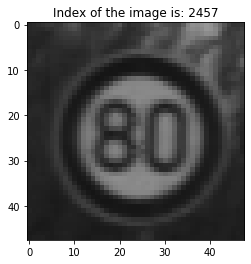
\includegraphics{sign.png}
  \caption{Road Sign}
  \label{fig:readsign}
\end{figure}


\subsection{Preparation}
The data is in the same range (0-255) so no scalling is needed. I experimented with minmax scaler and converted it to numbers between 0 and 1 but there was no accuracy improvement.
I also created a class column and attached the original numeric labels of the instances and attributes dataframe. 
Then I split the data into 70\% training and 30\% test data using scikit-learn's \parencite{scikitlearn} train\_test\_split. This is stratified, ensuring all labels are equally represented in the training and test data.
Reducing a dataset's dimensions increases accuracy. I used a model classifier that uses a RandomForestClassifier from scitkit\-learn to automatically detect which features are best in the dataset. The RandomForestClassifier uses many uncorrelated decision trees (in this case, 100). After the run I wound up with 576 features (25\%).


\section{Classification}
The data is imbalanced, meaning the labels each have different number of features associated with them. The classes are not represented equally. Here I used scikit\-learn's ComplementNB classifier as it's especially well suited for imbalanced data. I got a 71\% accuracy. As seen in the confusion matrix, it missed the third and eighth classes entirely classifying nothing in them (label 6 and 32), with a precision, recall and f1 score of 0 in each case.

\subsection{Naive Bayes}
\subsection{Bayesian Network Architectures}

\section{Clustering}
\subsection{k-means}
k-means works using the Expectation\-Maximization (EM) method. One has to specify the number of clusters we're looking for. In our case we have 10 labels, so 10 clusters. It found the clusters (see jupyter notebook), but it didn't match the label frequency count, and I had a hard time attaching a labels to the clusters.

\subsection{Tools for computation of optimal number of clusters}
Can we automatically determine the number of clusters?
For this I tried using scikit\-learn's MeanShift algorithm. It detects clusters automatically by updating a cluster with an instance that is closest to the mean of the cluster.
However it detected too many clusters to be useful, and produced data that wasn't informative.
\section{Research Question}
Q: Given data, is it possible to determine which data normalization method, which dimensionality reduction algorithm and which classification algorithm will work best with it?
\subsection{Genetic Programming}
This can be done using Genetic Programming \parencite{geneticprogramming}. TPOT \parencite{tpot} is an excellent Python package that implements GP for selecting the best pipeline given data and intended task. It's an AutoML \parencite{automl} implementation.
For our data it ran for about 5 hours with 5 generations, and produced a pipeline that gave 98\% accuracy, with the scikit\-learn's ExtraTreesClassifier as the classifier. Of not is that it did use the MinMaxScaller, so though for our data the models behave the same with 0-1 or the original 0-255 range data, scaling to 0-1 seems to be a best practice.
It achieved 100\% accuracy on two classes with the other at or above 95\%.


\printbibliography

\end{document}
